\documentclass{report}
\usepackage[utf8]{inputenc} % Prendre en compte les caractères accentués
\usepackage[francais]{babel} % Prendre en compte les particularités de la typographie française.
\usepackage{geometry}         % marges
\usepackage{graphicx}         % images
\usepackage{setspace}
\usepackage[french]{varioref}
\usepackage{titlesec}
\usepackage{parskip}
\usepackage{url}
\usepackage{verbatim}
\usepackage{caption}
\usepackage{enumitem}
\usepackage{ragged2e}
\usepackage{xcolor}
\usepackage{textcomp}
\usepackage{listings}
\usepackage{pgfgantt}
\usepackage{lscape}
\usepackage{pdfpages}

\lstdefinestyle{myLuastyle}
{
  language         = {[5.0]Lua},
  basicstyle       = \ttfamily,
  showstringspaces = false,
  upquote          = true,
  commentstyle     =\color{gray},
  stringstyle=\color{blue}
}

\lstset{style=myLuastyle}

\lstset{emph={%  
    ibm, addModel, getNumber, getModelValue, setModelValue, getName, addEvent%
    },emphstyle={\color{red}\bfseries}%
}

\newgantttimeslotformat{stardate}{%
	\def\decomposestardate##1.##2\relax{%
		\def\stardateyear{##1}\def\stardateday{##2}%
	}%
	\decomposestardate#1\relax%
	\pgfcalendardatetojulian{\stardateyear-01-01}{#2}%
	\advance#2 by-1\relax%
	\advance#2 by\stardateday\relax%
}

\titlespacing{\chapter}{0pt}{*-5}{*5}
\titlespacing{\section}{0pt}{*2}{*2}
\titleformat{\chapter}[hang]{\bf\huge}{\thechapter}{2pc}{}
%\titleformat{\chapter}[hang]{\bf\huge}{\thechapter}{14pt}{\LARGE}
\renewcommand{\baselinestretch}{1.2}
\setlength{\parskip}{1.5ex plus .4ex minus .4ex}
\setlength{\parindent}{15pt} 
\setlength{\topmargin}{-35pt}
\setlength{\textheight}{600pt}

\makeatletter
% subsubsubsection
\newcounter{subsubsubsection}[subsubsection] 
\renewcommand\thesubsubsubsection{\@roman\c@subsubsubsection}
\newcommand\subsubsubsection{\@startsection{subsubsubsection}{4}{\z@}%
                                     {-3.25ex\@plus -1ex \@minus -.2ex}%
                                     {1.5ex \@plus .2ex}%
                                     {\normalfont\small\bfseries}}
\newcommand*\l@subsubsubsection{\@dottedtocline{3}{5.2em}{1em}}
\newcommand*{\subsubsubsectionmark}[1]{}
\setcounter{secnumdepth}{2}
\makeatother

\begin{document}
\sloppy % Justification moins stricte : des mots ne dépasseront pas des paragraphes

\newcommand{\reporttitle}{Une extension du logiciel GVLE}     % Titre
\newcommand{\reportsubtitle}{Modélisation d'individu centré}     % SousTitre
\newcommand{\reportauthor}{Geneviève \textsc{Cirera} (SI4)} % Auteur
\newcommand{\reportsubject}{Rapport de Stage 4ème année} % Sujet
\newcommand{\HRule}{\rule{\linewidth}{0.5mm}}
\setlength{\parskip}{1ex} % Espace entre les paragraphes

\begin{titlepage}

\begin{center}

\begin{minipage}[t]{0.49\textwidth}
\vspace*{-2.4cm}
  \begin{flushleft}
    
\includegraphics [width=60mm]{images/LogoUNSA.jpg} \\[0.6cm]
    
  \end{flushleft}
\end{minipage} 
\begin{minipage}[t]{0.49\textwidth}
  \begin{flushright}
    
\includegraphics [width=60mm]{images/Logo_polytech_SI.jpg} \\[0.2cm]
  \end{flushright}
\end{minipage} \\[2.0cm]
\vspace*{-0.8cm}
\textsc{\Large Ingénieur en Sciences Informatiques}\\[0.5cm]
\textsc{\Large \reportsubject}\\[0.5cm]
\HRule \\[0.4cm]
{\huge \bfseries \reporttitle}\\[0.4cm]
{\Large \bfseries \reportsubtitle}\\[0.2cm]
\HRule \\[1.5cm]
\vspace*{-0.8cm}
\begin{minipage}[t]{0.64\textwidth}
  \begin{flushleft} \large
    \emph{Stagiaire :}\\
    \reportauthor
  \end{flushleft}
\end{minipage}
\begin{minipage}[t]{0.35\textwidth}
  \begin{flushleft} \large
   % \emph{Tuteur :} \\
    %M.~Frédéric \textsc{Precioso} \\[0.5cm]
    \emph{Maître de stage :} \\
    Patrick \textsc{Chabrier}
  \end{flushleft}
  \vspace*{1.0cm}
\end{minipage}
%\vspace*{7.0cm}
\textsc{\Large Entreprise INRA (Toulouse)}\\[0.5cm]
{\emph{16 juin 2014 - 20 septembre 2014}}\\
\vspace*{0.8cm}
\textsc{\Large Résumé}\\[0.5cm]
\justify
Résumé ici
\vfill

%{\large 5 mars 2012}
\center
\vspace*{0.3cm}

\includegraphics [width=50mm]{images/logoINRA.jpg} \\[0.6cm]
\end{center}

\end{titlepage}
 

\chapter*{Remerciements}
\setlength{\parskip}{2.5ex plus .4ex minus .4ex}
\setcounter{page}{2} 
Je tiens à remercier certaines personnes sans lesquelles ce stage n'aurait pas eu lieu.\\
Hélène Raynal, responsable du projet RECORD\footnote{Rénovation et CooRDination de la modélisation de cultures pour la gestion des agro écosystèmes}, Gauthier Quesnel du projet VLE\footnote{Virtual Laboratory Environment}, appartenants au département MIA\footnote{Mathématiques et Informatique Appliquées}.\\
Laurence Puillet et Olivier Martin, du projet Archimod, département PHASE\footnote{PHysiologie Animale et Systèmes d’Élevage} qui ont exprimé les besoins et sont les principaux futurs utilisateurs ainsi que Régis Sabbadin, Directeur de l'Unité MIAT\footnote{Mathématiques et Informatique Appliquées de Toulouse}, lieu de déroulement du stage.\\

Merci également à mon maître de stage Patrick Chabrier pour ses explications et conseils tout au long du stage ainsi que les stagiaires présents dans l'entreprise qui m'ont aidé et rendu le temps passé dans l'entreprise très agréable.\\

Je souhaite également remercier toutes les personnes au sein de l'école Polytech'Nice qui ont rendu ce stage possible.

\tableofcontents % Table des matières

\chapter{Introduction}
\setlength{\parskip}{2.5ex plus .4ex minus .4ex}
\section{Sujet de stage}
L'équipe-projet RECORD\footnote{Rénovation et CooRDination de la modélisation de cultures pour la
gestion des agro écosystèmes.} au sein de l'INRA\footnote{Institut National de la Recherche Agronomique} de Toulouse est une plate-forme de modélisation et de simulation informatique dédiée à l'étude des agro-écosystèmes.\\
Elle propose un ensemble d'outils logiciels: le logiciel VLE\footnote{Virtual Laboratory Environment}, rvle\footnote{utilisation d'un modèle depuis R}, pyvle\footnote{utilisation d'un modèle dans un script Python}, webrecord\footnote{outil d'interfaçage web des modèles} et une bibliothèque de modèles.\\
C'est un projet INRA ouvert à la communauté INRA et à ses partenaires.\\
\\
Le logiciel VLE repose sur le concept du formalisme DEVS\footnote{Discrete Event System Specification} qui fournis la notion de modèle abstrait. Il dispose d'extentions dont celle de Forrester qui permet de modéliser des individus en utilisant des diagrammes de Forrester. Cette fonctionnalité se présente sous la forme d'un plugin de modélisation qui, à partir d'un diagramme de Forrester, génère une classe C++ conforme au formalisme DEVS. Cette classe C++ implémente un système d'équations différentielles.\\
\\
Ce stage a pour but de fournir une solution intégrée et ergonomique permetant de ne pas modéliser un individu unique mais des populations d'individus.\\
Au cours de la simulation, les individus peuvent être manipulés (naissance, mort, vieillesse...) à l'aide d'évènements définis dans le plugin global qui devra être développé.

\section{Contexte}
Ce stage s'inscrit dans mon cursus universitaire pour clôturer ma 4ème année en ingénieurie informatique à Polytech'Nice Sophia.
Durant ce stage, j'ai travaillé de manière autonome au sein de l'équipe-projet RECORD sur un plugin global du logiciel VLE qui utilise le formalisme DEVS.\\
Ce formalisme est un formalisme modulaire et hiérarchique pour la modélisation, la simulation et l'analyse de systèmes complexes. Il existe deux types de modèle DEVS, le modèle couplé et le modèle atomique. \\
Le modèle couplé étant celui qui peut être formé par un ou plusieurs modèles atomiques et possède une dynamique exécutive.\\
Le modèle atomique, quant à lui, ne possède qu'une dynamique interne classique et des ports d'entrée et de sortie.\\
VLE permet de spécifier une dynamique, classique ou exécutive, à un modèle. La différence entre ces deux dernières est que la dynamique classique prend en considération des évènements en entré, effectue une ou plusieurs actions et renvoye des évènements en sortie au cours du temps alors que l'exécutive peut manipuler les modèles à l'intérieur d'un modèle couplé en plus de toutes les actions possibles par la dynamique classique.\\

\begin{minipage}{\linewidth}% to keep image and caption on one page
\makebox[\linewidth]{%        to center the image
  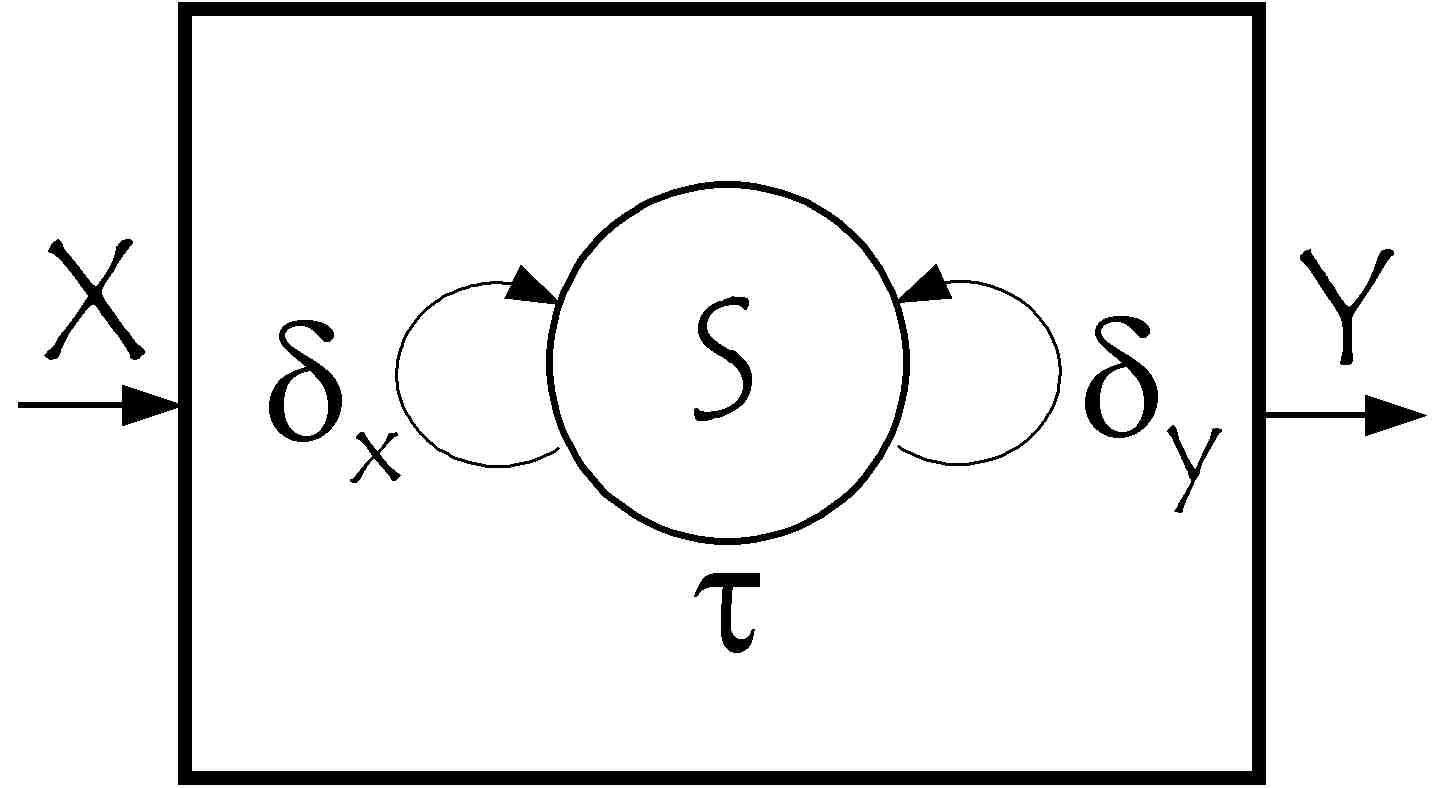
\includegraphics [width=60mm]{images/DEVSPP.jpg}}
\captionof{figure}{Dynamique DEVS}%\label{visina8}%      only if needed  
\end{minipage}

Dans ce schéma représentant le fonctionnement de DEVS, les entrées du modèle sont représentées par X, les sorties par Y, et $\delta_{x}$ la dynamique lors de la réception d'évènement, $\delta_{y}$ la dynamique interne du modèle c'est-à-dire ce qui arrive régulièrement au cours du temps $\tau$. S est l'état du système.


\include{context}

\chapter{Description du travail proposé}
\setlength{\parskip}{2.5ex plus .4ex minus .4ex}

\section{Expression des besoins}
\subsection{Besoins généraux}
Actuellement, le logiciel VLE permet de créer des individus un à un, de leur associer une dynamique, de les relier entre eux et de lancer des simulations. La dynamique de plusieurs individus peut être la même, et peut varier selon les conditions expérimentales qui décrivent les valeurs des paramètres si l'utilisateur les édite.\\
Cependant, il est nécessaire que l'utilisateur édite chaque individu un à un. Comment faire pour modéliser des troupeaux entiers sans avoir ce travail répétitif ~?\\
Pour l'instant, le logiciel VLE propose une interface pour créer la structure du système désirée par l'utilisateur. Puis, il doit programmer en C++ les classes qui définiront les dynamiques des modèles du système lui-même ou bien utiliser un plugin de modélisation comme Forrester par exemple.\\
Si l'utilisateur souhaite modéliser un troupeau, il faudra qu'il crée chaque individu un à un. C'est pourquoi, il était nécessaire de créer une extension du logiciel pour ces cas là. Une extension qui permettrait la création, suppression et la définition d'évènements sur les individus de manière simple et instinctive pour l'utilisateur.\\
L'utilisateur n'aurait donc plus besoin de programmer en C++ ni d'éditer des graphes et réutiliserait le plugin Forrester pour définir les classes d'individus qui serviront de base pour créer chaque individu lors de la simulation.

\subsection{Cas d'utilisations}
Un TP et un modèle type m'ont été donnés afin de me donner une idée des fonctionnalités attendues et de diriger la conception et le développement de mon plugin. Ces exemples ont été réalisés avec le logiciel Modelmaker.\\
Modelmaker est un logiciel de simulation de systèmes dynamiques, dont l'édition des modèles se fait par l'intermédiaire d'un diagramme de Forrester. Les modèles implémentables sont des systèmes d'équations différentielles.\\
Une des fonctionnalités qui nous a particulièrement intéressée dans le cadre du stage est la vectorisation des modèles pour partie ou en totalité qui permet en quelque-sorte d'émuler une approche de modélisation individu centré. D'autre-part, Modelmaker permet aussi de définir des événements qui, en fonction de l'état global du modèle, changent de façon discrète les valeurs des variables d'états. Il me fallait alors adapter les fonctionnalités proposées par Modelmaker afin que ce TP et modèle type soient réalisables avec VLE.\\
\\
Le TP avait pour but de créer 5 modèles dont chacun d'eux possédait un compartiment, le premier se vidant dans le deuxième et si le deuxième atteingnait une certaine valeur, se vidait immédiatement dans un troisième compartiment. Chaque modèle ayant des paramètres de vidange différents.\\
D'autres part, il devait être possible d'offrir à l'utilisateur la possibilité d'observer une ou plusieurs valeurs en particulier. Dans ce cas précis, la somme de tous les compartiments qui se vident.\\
\\
Le modèle type était plus complexe. Il s'agissait de faire naître 10 cellules à t=10, faire croître leurs poids suivant des paramètres distints puis à t=30, repérer la plus grosse cellule et faire décroître les 9 autres.\\ Lorsque la cellule la plus grosse atteint 0.99, 10 autres naissances sont lancées. Si une cellule a un poids inférieur à 0.1, la tuer.
 
\section[IBM] {IBM\footnote{Individual Based Model}}
\subsection{Paradigme IBM}
L'objectif est de pouvoir modéliser en spécifiant au sein d'un système dynamique des populations d'individus.\\
Un individu est formalisé par un système d'équations différentielles et tous les individus d'une population se réfèrent au même système d'équations différentielles.\\
Au sein d'une population les individus peuvent différer de par la valeur de leurs paramètres mais ce n'est pas une obligation.\\
\\
La dynamique des populations est définie par un ensemble d’événements portant sur les individus. Un évènement est défini par des conditions d'activation et des effets.\\
Les conditions d'activation sont exprimées en fonction du temps de la simulation ou de l'état du système simulé. L'état du système est l'union de tous les états des individus.\\
Il existe 3 types d'effet: Création d'un individu, suppression d'un individu et réinitialisation d'un individu.

\subsection{Structure du modèle DEVS}
Chaque individu est un système d'équations différentielles défini par une classe C++. Cette classe est appelée classe d'individu. C'est elle qui doit être défini par l'utilisateur puis qui servira de base pour créer tous les individus de ce type là. C'est pourquoi chaque individu de même type, a la même dynamique, seuls les paramètres peuvent varier entre eux si l'utilisateur souhaite en modifier un ou plusieurs.\\
Chaque individu est indépendant, ils n'intéragissent pas directement les un avec les autres. Ils doivent communiquer par l'intermédiaire d'un même controleur auquels ils sont tous connectés.\\
Chaque port de sortie de chaque individu est relié aux ports d'entrée du controleur, ce qui permet à ce dernier de recevoir des évènements, les traiter et envoyer des réponses adéquates par l'intermédiaire de ses ports de sortie reliés à chaque individu par des ports d'entrée.\\
Lors de la simulation, la dynamique du controleur se met en marche. Elle initialise tous les individus, exécute sa dynamique interne, reçoit les évènements externes et envoie des réponses aux individus. Durant la simulation, le controleur peut à tout moment, créer un nouvel individu, en supprimer ou en modifier les paramètres grâces aux évènements qu'il reçoit en entrée et qu'il peut envoyer en sortie.\\
Par exemple :\\
\noindent\begin{minipage}{\linewidth}% to keep image and caption on one page
\makebox[\linewidth]{%        to center the image
  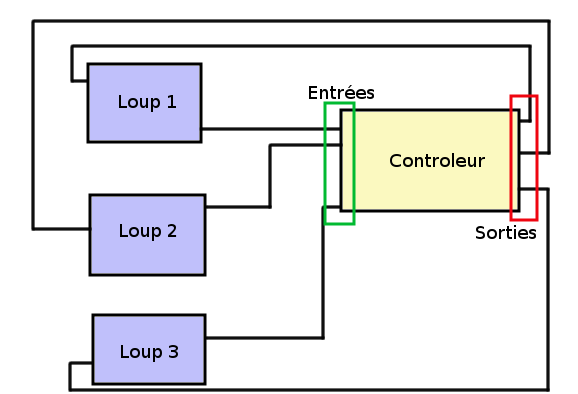
\includegraphics [width=150mm]{images/exemple_ibm.png}}
\captionof{figure}{Trois Loups créés par le controleur lors de la simulation}%\label{visina8}%      only if needed  
\end{minipage}

Le controleur crée les individus ``Loup 1'', ``Loup 2'' et ``Loup 3'' qui sont bien indépendants les uns des autres et tous reliés au controleur comme expliqué au paragraphe précédent. \\

\subsection{IBM dans VLE}
Dans VLE, chaque système ou simulation est représenté par un Vpz qui est un fichier xml où est décrit tout le système. Modèles présents (individus), conditions expérimentales (valeurs des paramètres), classes d'individus, ports d'entrées et de sorties...\\
Dans le Vpz, un controleur est obligatoirement présent s'il s'agit d'un système IBM. Il se crée automatiquement lors de la première ouverture du plugin IBM. \\Ensuite, les modèles souhaités par l'utilisateur sont créés lors de la simulation par le controleur grâce aux classes d'individu définies dans le vpz.\\
Par exemple : \\
\noindent\begin{minipage}{\linewidth}% to keep image and caption on one page
\makebox[\linewidth]{%        to center the image
  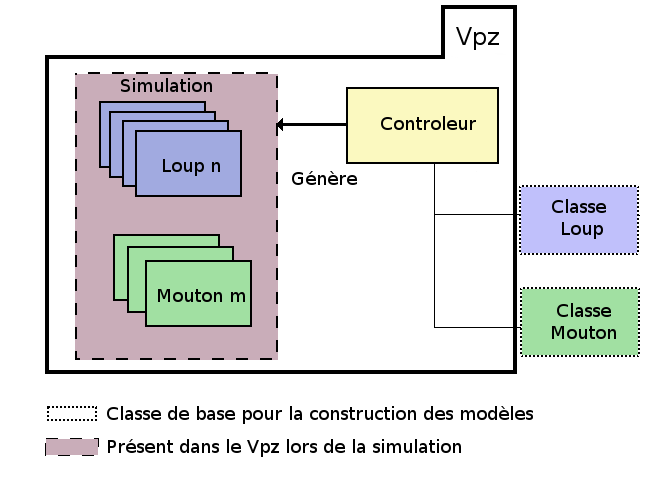
\includegraphics [width=160mm]{images/vpz1.png}}
\captionof{figure}{Composition d'un Vpz}%\label{visina8}%      only if needed  
\end{minipage}

Ici, le controleur crée n Loups et m Moutons lors de la simulation, mais seul le modèle ``Controleur'' est présent dans le vpz. Le controleur est cependant lié aux classes ``Loup'' et ``Mouton'' afin de pouvoir créer les individus.

\section{Fonctionnalités du plugin}
À son ouverture, le plugin récupère toutes les classes d'individu déjà présentes dans le Vpz. Il offre ensuite la possibilité d'ouvrir le plugin Forrester afin de créer d'autres classes et modifier ou supprimer les classes existantes.\\
Afin de manipuler les individus lors de la simulation, le plugin propose un champs de texte afin que l'utilisateur exprime ces besoins par l'intermédiare d'un petit langage simple appelé Lua et quelques extensions que j'aurai développées.\\
Ces besoins peuvent être multiple, ils peuvent avoir un effet sur les individus, création, suppression, modification ou bien renvoyer des informations, valeur d'une variable, nombre d'individus, identifiant d'un individu...\\
D'autre part, le plugin crée automatiquement un exécutive appelé ``Controleur'' à son ouverture. Controleur qui sera chargé de manipuler les individus selon le script qu'aura écrit l'utilisateur, et la dynamique DEVS.\\

\chapter{Description du travail réalisé}
\setlength{\parskip}{2.5ex plus .4ex minus .4ex}

\section{Architecture}
\subsection{Plugin global}
Afin de répondre au besoin, il a été décidé de développer un plugin global dans un paquet appelé vle.extension.ibm.\\
Un plugin global est une extension de logiciel permettant de mettre à disposition de l'utilisateur des fonctionnalités additionnelles. Cette extension se différencie d'un plugin classique par le fait qu'il ait accès au logiciel entier, à toutes ses informations, fonctionnalités...\\
Cependant, faire un plugin global a obligé quelques modifications des fichiers sources du logiciel. En effet, certaines informations étaient privées et il était nécessaire d'y accéder. Ce qui m'a obligé à bien comprendre la structure du logiciel grâce aux éléments que j'avais en main, fichiers sources et documentation, afin d'y insérer les bonnes méthodes correspondantes à mes besoins.

\subsection{Arguments}
Les raisons de cette décision sont variées. L'extension a besoin d'accéder à toutes les classes d'individu déjà créées par l'utilisateur précedemment dans le Vpz et qu'il puisse en créer de nouvelles depuis le plugin, afin que le clonage d'individu soit faisable. Le plugin a aussi besoin d'avoir accès au Vpz entier (conditions expérimentales, ports,...) et donc de VLE, car il intéragit avec ce dernier lors de la simulation.\\
De plus, une interface graphique du plugin devait être développée afin d'en faciliter l'utilisation, c'est pourquoi l'accès à GVLE\footnote{GUI pour VLE} était également indispensable.\\

Le plugin développé permet le lancement du plugin Forrester afin de créer les classes d'individu et est en lien avec un proxy permettant la communication entre le langage de script proposé à l'utilisateur et le controleur.\\

VLE est un logiciel fonctionnant grâce à des paquets, ils peuvent contenir un projet, un Vpz, une extension... Par exemple, le plugin Forrester fait parti du paquet vle.forrester, le plugin IBM est dans le paquet vle.extension.ibm.\\

\noindent\begin{minipage}{\linewidth}% to keep image and caption on one page
\makebox[\linewidth]{%        to center the image
  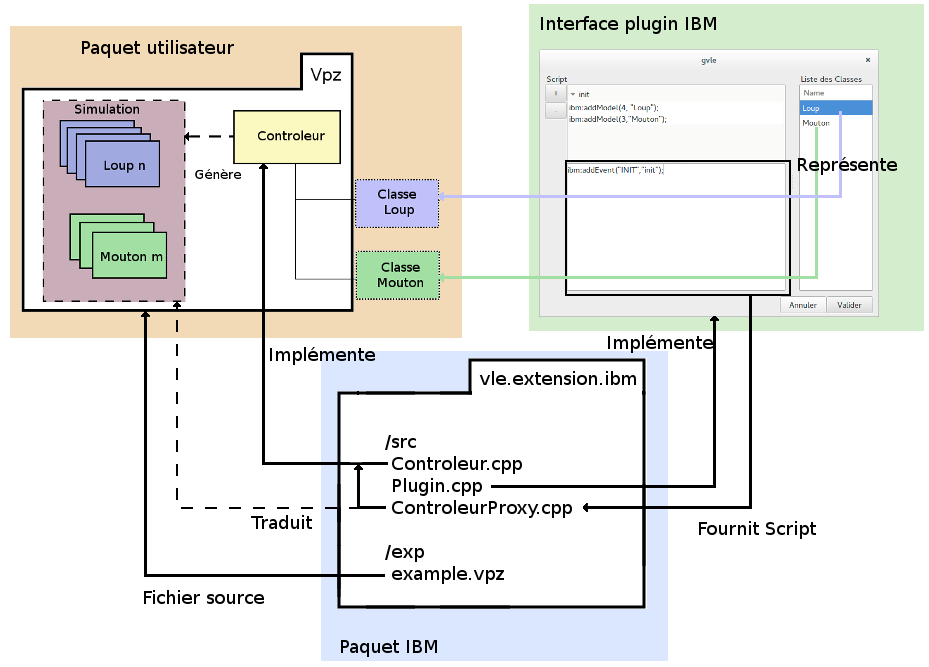
\includegraphics [width=150mm]{images/architecture.png}}
\captionof{figure}{Architecture du système}%\label{visina8}%      only if needed  
\end{minipage}

Ici, deux paquets, vle.extension.ibm en bleu et le paquet de projet de l'utilisateur en jaune. Le plugin IBM offre l'interface d'ibm où l'utilisateur décrit ses besoins puis il met en place le Controleur grâce à ces informations. Le Controleur peut alors générer les individus lors de la simulation.

\section{Controleur}
L'élément principal du système IBM est le controleur, il a pour but de gérer tous les évènements qui voyagent dans le système en les faisant passer par lui. Il hérite de nombreuses classes ce qui lui permet d'avoir les capacités d'une dynamique, d'un exécutive et d'un GenericAgent.\\
\noindent\begin{minipage}{\linewidth}% to keep image and caption on one page
\makebox[\linewidth]{%        to center the image
  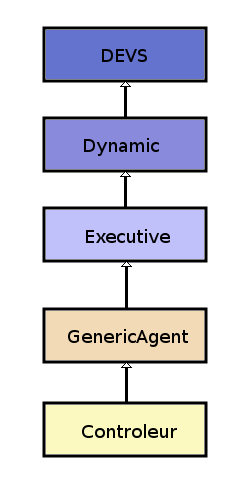
\includegraphics [width=60mm]{images/heritageControleur.png}}
\captionof{figure}{Graphe d'héritage du controleur}%\label{visina8}%      only if needed  
\end{minipage}

Il se crée automatiquement à la première ouverture du plugin IBM. Ces capacités sont multiples grâce à la hiérarchie d'héritage dont il est formé.
\subsection{Une dynamique}
Il possède la capacité d'une dynamique DEVS, recevoir des évènements par ses ports d'entrées, envoyer des évènements par ses ports de sorties, exécuter un programme interne à chaque pas de temps (transition interne), gérer les évènements externes (transition externe). Voici un résumé de sa dynamique. \\
\noindent\begin{minipage}{\linewidth}% to keep image and caption on one page
\makebox[\linewidth]{%        to center the image
  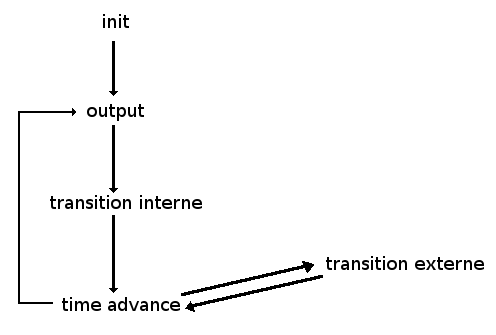
\includegraphics [width=100mm]{images/dynamiqueControleur.png}}
\captionof{figure}{Dynamique du controleur}%\label{visina8}%      only if needed  
\end{minipage}

Le controleur s'initialise dans init, puis exécute en boucle output, transition interne et time advance. \\
Output envoie les évènements par les ports de sortie, transition interne exécute les tâches régulières du controleur à chaque pas de temps t rendu par time advance.\\
La transition externe quant à elle s'exécute lors de la réception d'évènements, les traite puis la dynamique continue son cycle depuis time advance.

\subsection{Un executive}
Héritant d'Exécutive, le controleur a le pouvoir de créer des modèles mais aussi de les détruire et les modifier.\\
En effet, afin de créer des clones et les manipuler suivant les souhaits de l'utilisateur, le controleur a besoin de ces capacités.\\
Pour cela, un petit langage sera mis à la disposition de l'utilisateur afin qu'il puisse programmer les agissement du Controleur durant la simulation. \\
Ce petit programme est une chaine de caractère exécutée par le Controleur au bon moment grâce à sa dynamique afin de respecter les dates d'agissement souhaitées par l'utilisateur.

\subsection{Le scheduler}
Le Controleur hérite également de GenericAgent, ce qui lui donne accès à une sorte de calendrier. Il peut ainsi créer des évènements, les enmagasiner et exécuter les scripts envoyés par ces évènements à la bonne date.

\section{GUI}
Une interface simple a été développée pour l'utilisateur. Trois champs principaux en vert, rouge et les nuances de bleu ci-dessous.\\
La colonne de droite en vert qui liste toutes les classes d'individu présentes dans le Vpz ouvert. En survolant le nom d'une classe une infobulle s'ouvre pour afficher la liste des paramètres et compartiments de la classe en question, ce qui permet à l'utilisateur de programmer plus facilement. Il a directement accès à toutes les variables potentiellement modifiables au cours de la simulation.\\
Par un clique-droit sur la colonne des classes, un menu déroulant s'affiche où l'utilisateur peut décider de créer une nouvelle classe, modifier la classe sélectionnée ou la supprimer.\\
En rouge la zone de texte permettant l'écriture du script lua qui peut être des appels à évènements, des fonctions et/ou des initialisations de variables. Ce script n'est appelé qu'une fois en début de simulation.\\
En bleu, les évènements, on peut en ajouter grâce au bouton ``+'' sur le coté gauche ou en supprimer grâce au bonton ``-''. Le nom de l'évènement est en évidence après chaque flèche et le script correspondant est juste en dessous.\\

Ici l'exemple du tp Modelmaker sur le remplissage et vidange des compartiments.
Deux évènements, ``exec'' et ``init'', ``init'' est appelé lors de l'initialisation et le script de l'évènement ``exec'' tous les 0.1 à partir de la date 0.01.

\noindent\begin{minipage}{\linewidth}% to keep image and caption on one page
\makebox[\linewidth]{%        to center the image
  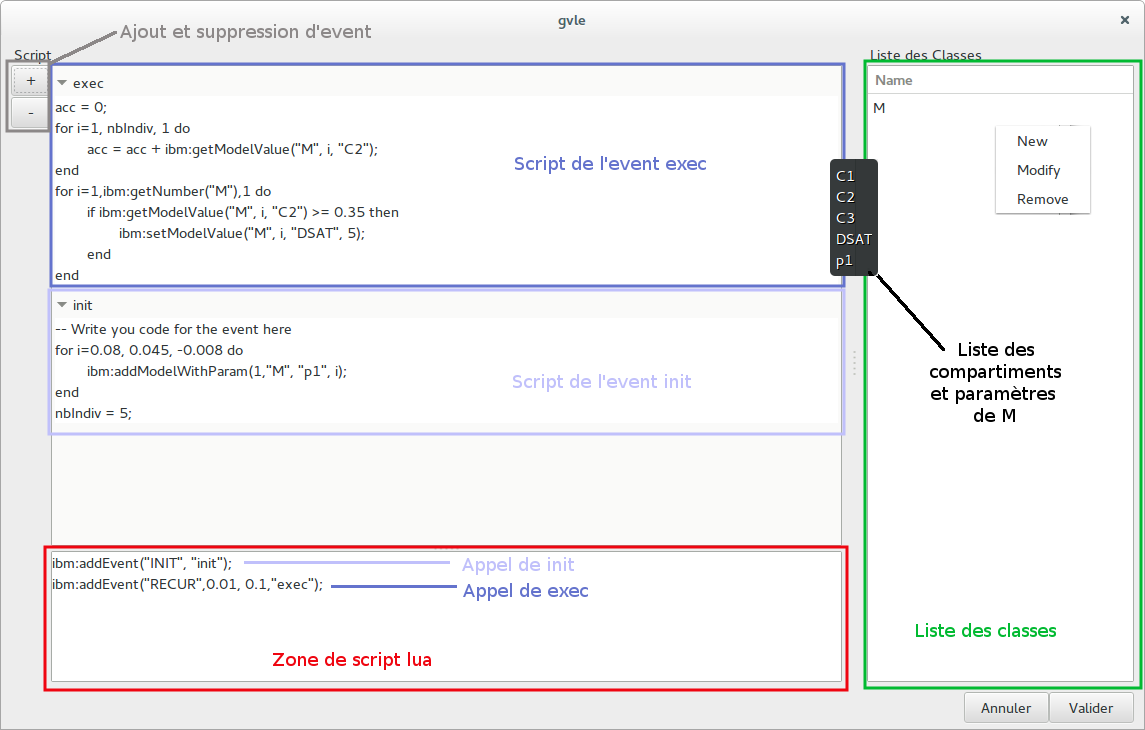
\includegraphics [width=150mm]{images/exemplePlugin.png}}
\captionof{figure}{Interface graphique du plugin IBM}%\label{visina8}%      only if needed  
\end{minipage}

\section{Lua \& addons}
Lua est un langage de script libre créé en 1993. Il a été conçu de manière à pouvoir être embarqué et augmenter les possibilités du système hôte.\\
Dans notre cas, il sert d'interprète entre ce que l'utilisateur souhaite faire et le controleur. Ainsi, on peut profiter de tout le langage lua, plus quelques fonctionnalitées que j'ai développées qui permettent certaines actions précises sur les individus.\\
\subsection{Mise en oeuvre}
Un script lua peut très facilement être exécuté depuis un programme C++. \\
On retrouvera les principales structures for, while, if, l'utilisation de variable... que l'utilisateur pourra se servir dans son script.\\
Mais ce langage ne permet pas à l'utilisateur d'effectuer des actions sur les individus. C'est pourquoi, des extensions à ce langage ont été développées et sont exécutées grâce à l'intermédiare d'un proxy.\\
\\
Dans l'exemple ci-dessous, le controleur récupère le script lua puis l'exécute. Comme addModel n'existe pas dans le langage lua, le proxy comblera cette anomalie en appelant la fonction du controleur associée à addModel à chaque fois qu'elle sera appelé. Dans ce cas, trois fois.\\

\noindent\begin{minipage}{\linewidth}% to keep image and caption on one page
\makebox[\linewidth]{%        to center the image
  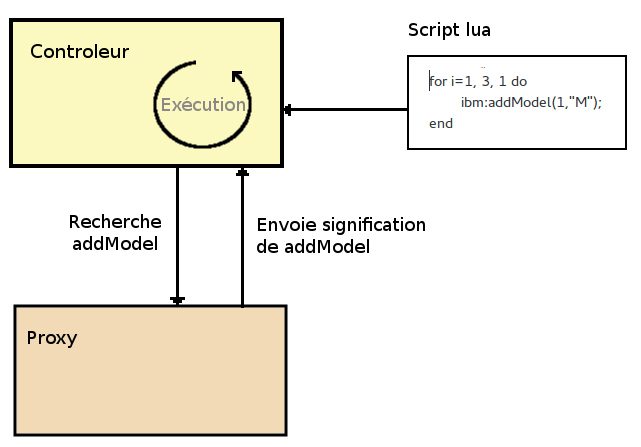
\includegraphics [width=150mm]{images/proxyLua.png}}
\captionof{figure}{Exécution d'un script lua depuis le controleur}%\label{visina8}%      only if needed  
\end{minipage}

\subsection{Les extensions}
Chaque extension du langage lua ont comme préfixe ``ibm\string:''. Elles permettent d'avoir des effets sur les modèles, d'obtenir des informations ou lancer des évènements.\\
Voici la liste des extensions développées qui ont des effets sur les individus :
\begin{itemize}[label=\textbullet,font=\large]
	\item addModel(n,``M'')\\
	Ajoute n model de type ``M''.
	\item delModel(``ModelName'')\\
	Supprime le modèle dont le nom est ``ModelName''.
	\item addModelWithParam(n, ``Class'', ``Param1'', value1, ``Param2'', value2, ...)\\
	Ajoute n model de type ``Class'' en modifiant les paramètres de telle manière à ce que Param1 = value1 et Param2 = value2. Le nombre de paramètre à modifier est indéfini.
	\item setModelValue(``class'', i, ``varName'', varValue)\\
	Modifie la valeur de ``varName'' par ``varValue'' du i\up{ème} modèle de la classe ``class''.
	\item setModelValue(``modelName'', ``varName'', varValue)\\
	Modifie la valeur de ``varName'' par ``varValue'' du modèle nommé ``modelName''.
\end{itemize}
Les extensions qui permettent d'avoir des informations sur les individus.
\begin{itemize}[label=\textbullet,font=\large]
	\item getModelValue(``modelName'', ``varName'')\\
	Renvoie la valeur de la variable ``varName'' du modèle dont le nom est ``modelName''.
	\item getModelValue(``class'', i, ``varName'')\\
	Renvoie la valeur de la variable ``varName'' du i\up{ème} modèle de la classe ``class''.
	\item getModelName(``class'',i)\\
	Renvoie le nom du i\up{ème} modèle de la classe ``class''.
	\item getNumber(``class'')\\
	Renvoie le nombre d'individu de la classe ``class''.
	\item getTime()\\
	Renvoie la date actuelle durant la simulation.
\end{itemize}

Dans toutes ces extensions, il est possible de remplacer la valeur des quantités, double ou int, par une chaîne de caractère qui correspond à un paramètre des conditions expérimentales du controleur.\\
Quantité de modèles ajoutés dans addModel, la quantité de modèles et la valeur des paramètres dans addModelWithParam et la valeur de ``varValue'' dans setModelValue.\\

L'extension permettant de lancer des évènements est addEvent. Cette fonction peut être de trois types, ``INIT'', ``SINGLE'' ou ``RECUR'' précisé en premier paramètre. \\
L'évènement lancé se traduit par l'exécution d'une fonction écrite par l'utilisateur dans le script. Cette fonction est toujours précisé en dernier paramètre de addEvent.\\
``INIT'' permet de lancer un premier script à l'initialisation de la simulation.\\
``SINGLE'' permet de lancer un évènement ponctuel dans la simulation, c'est-à-dire l'exécution d'une fonction lua à un temps déterminé par l'utilisateur. La syntaxe sera addEvent(``SINGLE'', date, ``fonction'').\\
``RECUR'' permet de lancer un évènement qui s'exécutera à une certaine fréquence depuis une date déterminée par l'utilisateur. On aura addEvent(``RECUR'', date, frequence, ``fonction'').\\

Par exemple, ici deux évènements sont implémentés.\\
Initialisation, 5 loups sont créés avec un age entre 1 et 5.

%\noindent\fbox{\begin{minipage}{1.0\textwidth}
%- -Event init\\
%for i=1,5,1 do\\
%	\textcolor{red}{ibm\string:addModel}(``nbLoup'',``Loup'',``age'',i);\\
%end
%\end{minipage}}

\begin{lstlisting}[frame=single]
--Event init
for i=1,5,1 do
	ibm:addModel("nbLoup","Loup","age",i);
end
\end{lstlisting}

Ici, l'évènement ``dyn'' ajoute 1 à l'age de chaque loup. Ceux qui atteignent 10 sont affichés.
\begin{lstlisting}[frame=single]
--Event dyn
for i=1,ibm:getNumber("Loup"),1 do
	x = ibm:getModelValue("Loup",i,"age")
	ibm:setModelValue("Loup",i,x + 1)
	if ibm:getModelValue("Loup",i,"age") == 10 then
		print(ibm:getName("Loup",i))
	end
end
\end{lstlisting}

Appel des évènements. Tout d'abord ``init'' à l'initialisation puis l'évènement ``dyn'' à partir de la date 4 et tous les 1 jusqu'à le fin de la simulation.

\begin{lstlisting}[frame=single]
ibm:addEvent("INIT","init");
ibm:addEvent("RECUR",4,1,"dyn");
\end{lstlisting}

En rouge, toutes les extensions utilisées dans le script.

Une autre fonctionnalité a été implémentée afin de permettre à l'utilisateur d'observer les variables de son choix faisant partie de son script lua.\\
Par exemple, l'utilisateur peut observer la quantité d'individus au cours de la simulation en définissant une variable globale ``var'' dans le  script d'un évènement appelé récursivement qui prendrait pour valeur la somme de tous les individus.\\ Puis l'utilisateur doit déclarer cette variable ``var'' dans les observables du Controleur et lui associer une vue de sortie. Il sera alors possible d'observer la quantité d'individus tout au long de la simulation.
\section{Déroulement du stage}
\subsection{Découverte}
Les premiers jours ont été destinées à l'installation de toutes les parties nécessaires au fonctionnement du logiciel et à la compréhension de ce dernier, à quoi sert-il et comment fonctionne-t-il du point de vue de l'utilisateur.\\
\\
Durant cette phase, j'ai lu la documentation associée à l'utilisation du logiciel afin de comprendre comment était représenté un individu, comment une simulation fonctionnait, l'envoie de messages entre modèles...\\
De plus, j'ai effectué un TP destiné à apprendre à utiliser le plugin Forrester, lancer des simulations et observer les valeurs de certains paramètres.\\
J'ai également réalisé à la main le clonage d'un individu en modifiant un de ses paramètres afin d'avoir une idée plus claire de ce qu'on attendait de moi durant ce stage.
\subsection{Langage de script}
Il était dès le départ évident que l'utilisateur devra programmer une petite partie afin de décrire la vie des individus qu'il aura créé.\\
J'ai tout d'abord commencé à développer les extensions de lua décrites précédemment par l'intermédiaire d'un parser en C++ dans le controleur sans le langage lua. Et seules ces fonctionnalités pouvaient être appelées.\\
Cette méthode était très limitée, c'est pourquoi l'insertion d'un langage existant était nécessaire.\\
Lua, un langage de programmation très simple, se mélange parfaitement au C++ et permet une plus grande liberté à l'utilisateur. Créant un proxy afin de faire l'intermédiaire entre lua et les fonctions C++, l'utilisateur peut profiter de tous les avantages et multiplier ces possibilités.\\
Après la mise en place du proxy, le développement de nouvelles extensions s'est faite sans difficultés.
\subsection{La dynamique}
Après avoir pris connaissance du logiciel et ses fonctionnalités, il m'a fallu comprendre la dynamique de fonctionnement c'est-à-dire la dynamique DEVS. Elle se traduit par l'ordre dans l'exécution des fonctions dans une dynamique, reception d'évènement, envoie d'évènement, transition interne et externe...\\
A la base, l'utilisateur devait programmer deux script, un pour l'initialisation et un autre qui s'exécutait en continu en transition interne. \\
Cependant, j'ai été confronté à un problème. L'utilisateur ne pouvait pas décider d'exécuter une commande à un moment déterminé au cours de la simulation, par exemple si l'utilisateur souhaite faire naître deux loups à la moitié de la simulation. Pour cela, il devait passer par l'intermédiaire de booléen, ce qui compléxifiait énormément le code et le ralentissait.\\
Afin de résoudre se problème, j'ai mis en place un Scheduler. Il permet l'ordénation d'évènements par le temps auxquel ils doivent s'exécuter puis l'envoie de ses derniers à la bonne date lors de la simulation.\\
Grâce au scheduler, l'utilisateur simplifie son code en ne faisant que des fonctions lua puis appelle ses dernières dans l'ordre et la fréquence qu'il souhaite grâce à la commande d'ajout d'évènement addEvent.
\subsection{Bugs \& tests}
Au cours du développement, de nombreux bugs se sont manifestés. Leurs résolutions étaient parfois évidente, mais il pouvait aussi être plus difficil de trouver leurs sources. En effet, ils étaient parfois dû à mon propre code, mais travaillant sur une version en développement, les bugs pouvaient cependant être dû à l'instabilité de l'application. C'est pourquoi, j'ai effectué des rapports de bug.\\

Afin de repérer les sources d'erreurs plus facilement, j'ai utilisé gdb, mais parfois ce système ne fonctionnait pas car c'était gdb lui-même qui provocait les bugs.\\
D'autres bugs n'étaient visibles que lors de l'analyse des résultats obtenus après simulation. Pour remonter jusqu'aux erreurs, il a fallu songer à des tests, des scripts lua plus simples mais qui pourtant reproduisaient le bug.\\
Après avoir réalisés ces tests, les plus pertinents ont été insérés dans le paquet vle.extension.ibm avec les TP donnés à titre d'exemple des besoins, afin que l'utilisateur en téléchargeant le plugin, puissent avoir des exemples d'implémentations simples.

\subsection{Outils \& organisation}
J'ai développé le plugin vle.extension.ibm par l'intermédiaire de gedit de manière totalement libre grâce à au gestionnaire de version GIT et le dépôt Github.\\
Nous avons fait une prémière réunion avec l'équipe-projet Record afin de clarifier ce que je devrais développer en début de stage. Des réunions très régulières avec mon tuteur ont eu lieu dans le but de vérifier mon avancée et envisager les possibilités futures de développement.\\
De plus, j'avais à ma disposition des User Stories qui décrivaient ce que l'utilisateur devait pouvoir réaliser avec le plugin afin de me diriger dans mon développement. Ces User Stories étaient progressives, elles partaient de fonctionnalités simples comme afficher le bouton de démarrage du plugin à la mise en place de Scheduler.\\
Afin de vérifier que toutes les fonctionnalités étaient bien mise en place, j'ai modélisé les systèmes demandés dans les deux TP des besoins, croissance des cellules et vidange des compartiments. 

\chapter{Conclusion}
\setlength{\parskip}{2.5ex plus .4ex minus .4ex}
%1. Ce que le stage m'a apporté
%2. Logiciel fonctionnel..
%Ce qui reste, tests fonctionnel, de performance
Grâce à ce stage, j'ai pu voir comment développer de nouvelles fonctionnalités à partir de besoins précisés en début de stage. Ces besoins s'attachaient à un logiciel existant, il a donc fallu apprendre à lire et comprendre le fonctionnement avant toute modification et/ou ajout de code.\\
J'ai également pu voir plusieurs aspects de développement, créer un plugin sur un logiciel existant, créer les fonctionnalités de ce plugin, créer son interface graphique mais aussi l'aspect debuguage, rapport de bug du logiciel existant et debuguage de mon propre code.\\
Ce stage m'a apporté des compétences telles que le moyen de répondre à un besoin, de rechercher des informations, mais aussi des compétences techniques notamment en C++.\\

A la fin de ce stage, le plugin développé est fonctionnel, les usagés peuvent s'en servir afin de modéliser des individus dans le sens IBM.\\
Ce plugin fournit de nouvelles possibilités que VLE ne pouvait pas offrir auparavant. Cependant, du travail reste à faire comme des tests sur les fonctionnalités. En effet, le plugin répond actuellement aux besoins cités en première partie mais peut-être que de nouveaux cas d'utilisation sont à venir et de nouvelles fonctionnalités seraient nécessaires comme par exemple faciliter l'inclusion de modèle IBM dans d'autres modèles, proposer à l'utilisateur une interface afin qu'il choisisse les ports d'entrée et de sortie qui lui sont nécessaire...\\
De plus, certaines fonctionnalités comme l'observation de variable globale est possible mais aucune interface graphique n'a été développée.\\


\chapter{Bibliographie}
\noindent Documentation de VLE :\\
\url{http://www.vle-project.org/doxygen/dev/}\\
\vspace{0.5cm}

\noindent Tutorials VLE :\\
\url{http://www.vle-project.org/wiki/Tutorials}\\
\vspace{0.5cm}

\noindent Documentation utilisateur GVLE :\\
\url{http://record-elearning.inra.fr/record/}

\chapter{Abstract}
I did this internship with the RECORD team in the National Institute for Research Agronomics in Toulouse, a french institute founded in 1946.\\
I learnt the DEVS dynamics using VLE software. After that, I autonomously started develop a software extension in C++ programming language to provide new features to GVLE software. The objective is to give new modelisation possibilities to the user like cloning and manage individuals during a simulation.\\
I saw differents aspects of developpement: the definition of the users needs, developpement of functionalities, grafic interface, debug, tests...

\chapter{Annexe}
\setlength{\parskip}{2.5ex plus .4ex minus .4ex}
%Exemple de US
\section{Exemple de User Story}
\noindent\begin{minipage}{\linewidth}% to keep image and caption on one page
\makebox[\linewidth]{%        to center the image
  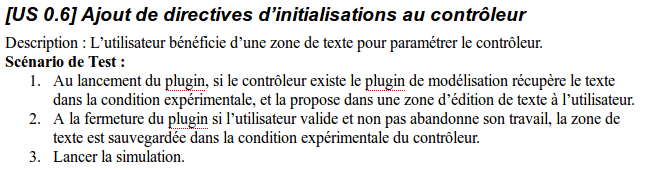
\includegraphics [width=130mm]{images/exempleUS.png}}
\captionof{figure}{Exemple de User Story}%\label{visina8}%      only if needed  
\end{minipage}

\appendix

\end{document}
